\documentclass[12pt, twoside]{article}
\usepackage[letterpaper, margin=1in, headsep=0.5in]{geometry}
\usepackage[english]{babel}
\usepackage[utf8]{inputenc}
\usepackage{amsmath}
\usepackage{amsfonts}
\usepackage{amssymb}
\usepackage{tikz}
\usetikzlibrary{quotes, angles}
\usepackage{graphicx}
%\usepackage{pgfplots}
%\pgfplotsset{width=10cm,compat=1.9}
%\usepgfplotslibrary{statistics}
%\usepackage{pgfplotstable}
%\usepackage{tkz-fct}
%\usepackage{venndiagram}
\usepackage{enumitem}
\usepackage{multicol}

\usepackage{fancyhdr}
\pagestyle{fancy}
\renewcommand{\headrulewidth}{0pt} % disable the underline of the header

\fancyhead[RO]{Name: \hspace{1.5in}}
\lhead{BECA / Dr. Huson / 10th Grade Geometry\\* 4 December 2018}

\begin{document}
\subsubsection*{Classwork: Triangle congruence proofs}
 \begin{enumerate}

  \item Given $\triangle ABC$ and $\triangle EFG$ with $\angle A \cong \angle E$, $\overline{AB} \cong \overline{EF}$, and $\overline{AC} \cong \overline{EG}$. Prove $\triangle ABC \cong \triangle EFG$.\\[0.5cm]
    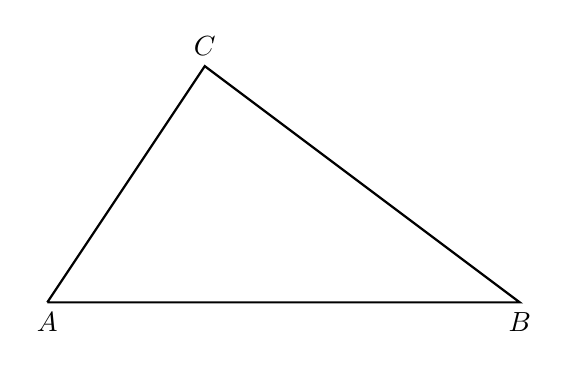
\begin{tikzpicture}
        \draw [thick]
          (2,0)node[below]{$A$}--
          (8,0)node[below]{$B$}--
          (4,3)node[above]{$C$} --(2,0);
      \end{tikzpicture}
      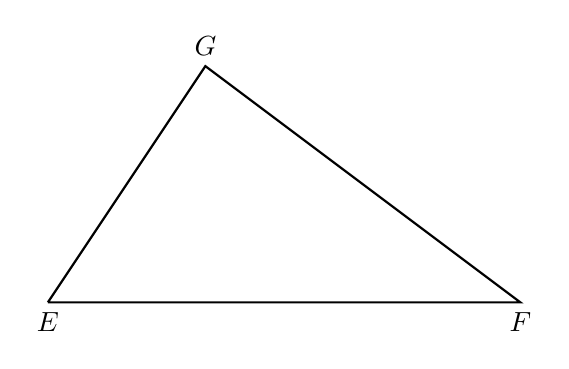
\begin{tikzpicture}%[scale=0.7]
        \draw [thick]%(0,0)node[below]{$A$}--
        (2,0)node[below]{$E$}--
        (8,0)node[below]{$F$}--
        (4,3)node[above]{$G$} --(2,0);
    \end{tikzpicture}

    \begin{multicols}{2}
      \underline{Statement} \\
      \underline{Reason}
    \end{multicols}
    \begin{multicols}{2}
      \raggedcolumns
      \begin{enumerate}[label={\arabic*)}]
        \item $\triangle ABC$, $\triangle EFG$
        \item $\angle A \cong \angle E$
        \item $\overline{AB} \cong \overline{EF}$, and $\overline{AC} \cong \overline{EG}$
        \item $\triangle ABC \cong \triangle EFG$ \\
      \end{enumerate}
      \begin{enumerate}[label={\arabic*)}]
        \item Given
        \item \rule{4cm}{0.15mm}
        \item \rule{4cm}{0.15mm}
        \item \rule{4cm}{0.15mm}
      \end{enumerate}
    \end{multicols}

  \item Given $\triangle ABP$ and $\triangle JKP$ with $\angle A \cong \angle J$ and $\overline{AP} \cong \overline{JP}$. Prove $\triangle ABP \cong \triangle JKP$.\\[0.5cm]
    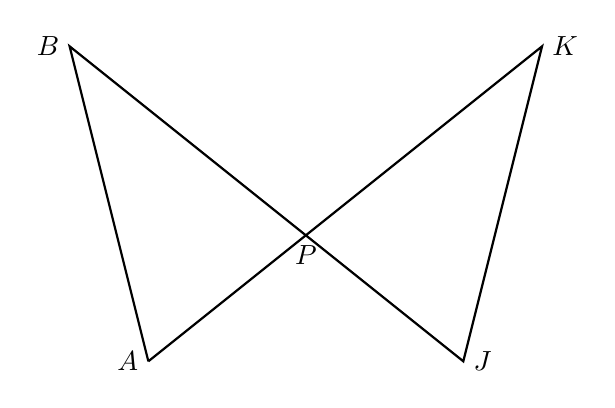
\begin{tikzpicture}
        \draw [thick]
          (-2,-1)node[left]{$A$}--
          (3,3)node[right]{$K$}--
          (2,-1)node[right]{$J$}--
          (0,0.6)node[below]{$P$}--
          (-3,3)node[left]{$B$}--(-2,-1);
      \end{tikzpicture}

    \begin{multicols}{2}
      \underline{Statement} \\
      \underline{Reason}
    \end{multicols}
    \begin{multicols}{2}
      \raggedcolumns
      \begin{enumerate}[label={\arabic*)}]
        \item $\triangle ABC$, $\triangle JKP$
        \item \rule{4cm}{0.15mm}%$\angle A \cong \angle J$ and $\overline{AP} \cong \overline{JP}$ %\vspace{0.4cm}
        \item $\angle APB \cong \angle JPK$ %

        \item $\triangle ABP \cong \triangle JKP$
      \end{enumerate}
      \begin{enumerate}[label={\arabic*)}]
        \item Given
        \item Given
        \item \rule{4cm}{0.15mm}
        \item \rule{4cm}{0.15mm}
      \end{enumerate}
    \end{multicols}

\newpage
\subsubsection*{List of theorem/situations for $\triangle \cong$ proofs}
  \item Vertical angles w segment bisectors
  \item Transversal corresponding
  \item Transversal with shared side on transversal
  \item Two inscribed in circle with vertical angles
  \item Inscribed in circle triangle with external angle, showing arc measure relationship
  \item Rotate triangle


\end{enumerate}
\end{document}
